\documentclass[11pt, twocolumn]{article}

\usepackage{amsmath}
\usepackage{amssymb}
\usepackage{graphicx}
\usepackage{booktabs}
\usepackage{fancyvrb}

\newcommand{\MARCUS}[1]{}

% GET RID OF AS MANY "WE FEEL"s AND "WE THINK"s AS POSSIBLE

\begin{document}
\title{The Effectiveness of Brightness Metrics for Ball Detection}
\author{Marcus Christiansen, Will Gantt}
\maketitle

% NEED TO INCLUDE RESULTS FROM HEMISPHERE TESTS IN THE PLACES MARKED BELOW
\abstract{\textbf{Broadly, the goal of this project was to determine whether brightness measurements could be an effective tool for ball detection. Specifically, we considered how such metrics might be incorporated into the spot filter; first, in the identification of blacks spots, second, in a comparison between the brightness values of the top and bottom hemispheres of the ball itself, and, third, in a comparison between the brightness values of the regions immediately above and below the ball. Regarding black spots, we found that there is little difference in brightness between true and false positive instances. In the comparison of hemispheres, we found that \MARCUS{Results here} \ldots. In the comparison of above-ball and below-ball regions, we saw \MARCUS{Results here} \ldots.}

\section{Overview}
Since the recent decision of the RoboCup Standard Platform League to replace the standard orange ball with one more reminiscent of a classical soccer ball, teams have been faced with a slew of new vision challenges. As the ball's primary color is now white, teams must find novel ways to distinguish it from other white objects, including field lines, goal posts, and robots. Furthermore, they must differentiate the black pentagons of the ball from such things as robot joints and other dark spots on the field. Thus, color alone can no longer serve as a reliable marker of the presence of a ball. Consequently, the Northern Bites have implemented a variety of additional checks. These include determining the expected radius of the ball at different locations on the field, evaluating the spatial relationships between black spots, and verifying that a candidate ball is in fact on the field. \\
\indent Although the ball detector concerns itself to a great extent with white and black, it makes almost no use of brightness inputs. Since black is notoriously difficult to characterize strictly on the basis of color (U- and V-) values, we wanted to see whether brightness (Y-values) could provide some helpful information in this regard. 

\section{Experiment}
Currently, the Northern Bites robots identify candidate balls using a spot filter. The basic principle consists in scanning an image with a ``filter,'' which comprises a small, square-shaped region nested within a larger one. At each position in the scan, the filter performs a simple check to determine whether the outer region is whiter on average than the inner one. The idea is that a ball will tend to be darker in the middle, since the black spots typically fall closer to its center, and whiter around the edges. \\
\indent The tests we ran operated on spots that the detector already identified. That is, the tests were intended to filter, rather than discover, candidate balls. The first test considered the median Y-value of each detected black spot, with the goal of determining whether there was any consistent, significant difference between true positives (black spots actually on the ball) and false positives. The second compared the median Y-values of the top and bottom halves of the inner region of a white spot (a candidate ball). We reasoned that, because the field is lit from above, the top half of a ball should tend to be brighter than the bottom half. By the same logic, we hypothesized that the shadow cast by the ball on the field itself should render the area of the field directly below the ball darker than the area directly above it. This was implemented as a third test. \\
\indent All three tests were conducted on logs taken in the robotics lab at illuminance levels of 150, 300, and 450 lux.\footnote{In truth, measuring the brightness of an entire room with this level of accuracy is impossible, given imperfections in the light meter, as well as minor fluctuations in the illumination of the room itself. These values should therefore be taken as approximate.} For each level, we placed the robot in 12 different scenarios, and for each scenario, we made adjustments to some combination of the following variables:
\begin{itemize}
\item The presence of the ball on the field (i.e., \emph{whether} the ball is on the field)
\item The ball's position on the field.
\item The robot's distance from the ball.
\item The robot's position on the field.
\item The number of other robots present on the field.
\end{itemize}
\subsection{Black Spot Detection}
In the first test, we differentiated true and false positive black spots by looking at the output of the ``DebugImageView'' module in the tool, which circles in yellow all of the black spots that the ball detector has identified. For each log, we documented the total number of black spots detected, the number of true positives, the number of false positives, the Y-values of each spot, the number of other robots on the field, and the presence of the ball in the image. Once we had obtained this information for all logs at a given illuminance level, we calculated the median, mean, and standard deviation of the true and false positives.
% THESE SECTIONS NEED TO BE FILLED IN
\subsection{Hemisphere Comparison}
\subsection{Region Above and Below Ball}

\section{Algorithm}
As our goal in this project was merely to see whether brightness tests could be used effectively in the ball detector, and not to write game-ready code, we were not particularly concerned with algorithmic efficiency. We do, however, offer suggestions for how the most promising of these algorithms might be improved. The source code for the functions we used can be found at the end of this paper, but we have included high-level descriptions of what each does below.
\begin{description}
\item[\texttt{getMedianBrightness}:] A spot consists of a smaller square region nested within a larger one. This function determines the median Y-value of the inner region of a black spot by simply iterating over all of the pixels in that region, and adding the Y-value of each to a vector. The vector is then sorted and the element at the median index is returned.
\item[\texttt{topOfBallBrighterThanBottom}:] Takes the inner region of a ball (a white spot) and divides it into a top half and a bottom half. The median Y-values of each half are determined using the same method as in \texttt{getMedianBrightness}, and are returned together as a pair of doubles.
\item[\texttt{aboveBallBrighterThanBelowBall}:] This uses the same basic approach as the previous function but considers the rectangular areas (1) between the top edge of the outer region of the spot and the top edge of the inner region, and (2) between the bottom edge of the outer region and the bottom edge of the inner region. Both of these areas cover some of the ball, as well as some of the field. The function determines the median Y-values of each region and returns them as a pair of doubles. 
\end{description}

\section{Results}
Unfortunately, neither of us has the knowledge required to conduct tests for the statistical significance of our results. Despite this, we are willing to conclude, based on the similar averages and large standard deviations of the Y-values of true and false positive black spots (shown in Figure \ref{fig:table} at the end of this paper), that brightness is not an effective feature for making this distinction.\\
\indent \MARCUS{YOUR RESULTS HERE} Results from hemisphere test \ldots \\
\indent \MARCUS{YOUR RESULTS HERE} Results from above-ball/below-ball test \\
\indent Our experiments have at least shortcomings that we want to acknowledge. For one, the measurements provided for the level of illuminance in the lab are only rough approximations. Although we did our best to eliminate outside light sources and to accurately calibrate the light meter, we cannot guarantee that the illuminance level remained fully consistent across trials. We suspect that complete consistency in this respect would not have had a significant impact on the results of the hemisphere comparison or above-ball/below-ball tests. It is conceivable, however, that it would have had some effect on the black spot experiment in that it perhaps would have yielded a slightly more consistent difference between true and false positives. \\
\indent For another, the experiments suffer from a lack of diversity in the data collected. All of our logs were taken at a single location --- to wit, the RoboCup lab. We are confident that the hemisphere comparison test is sufficiently robust to work under a variety of lighting conditions, but we would like to have more data to support the claim. Regarding black spots, however, if the robot cannot distinguish the true from the false under lab conditions, we doubt that it would perform much better elsewhere.

\section{Future Work}
Clearly, there is much work that remains to be done on the Northern Bites' ball detection system. The results of our experiment suggest several problems particularly in need of attention. \\
\indent First, the system is remarkably fragile. By this, we mean that even the slightest change in visual input can result in radically different output. Our comparison of logs taken in the same scenario under the same lighting conditions made this apparent. The differences between these logs are imperceptibly minor, and yet they would routinely produce outputs that disagreed on such important judgments as whether a ball was present in the image, how many black spots there were, and where those spots were located. Figure \ref{fig:logs} in the appendix provides a nice illustration of the problem. \\
\indent Second, the \texttt{processDarkSpots} function in \texttt{BallDetector.cpp}, which calls all of the filtering functions for black spots, should have a hard upper limit on the number of candidate black spots allowed to remain as candidates after it has been called. One might reasonably expect the presence of other robots in the image to increase the number of false positives detected, but in several instances, the tool marked more than 10 identified black spots, and in a couple of the cases, the figure exceeded 25 spots (see Figure \ref{fig:fpBlackSpots}). We can conceive of no practical circumstance in which a robot would benefit from information on this many spots \emph{after} the filters have already been run. We suggest that \texttt{processDarkSpots} limit itself to returning only the three spots for which it has the highest confidence. \\
\indent Third, the detector struggles to locate balls when they are on a field line and when they are more than a couple meters away. Neither of these is a new problem, but given the relative frequency with which a robot is likely to encounter one of these situations, it is imperative that we find a way of dealing with them. The hemisphere comparison may offer some help in the former case, but additional methods would be of great use. \\
\indent Fourth, and as a corollary to the previous remark, the problem of detecting balls in the first place ought to be given greater priority than the problem of eliminating false ones. On the whole, we saw many more false negatives than false positives. Regardless of whether one thinks it is better to see no balls at all than to see a false one, this is a shortcoming of the system that should be addressed immediately. \\
\indent Fifth, and finally, in light of the promising results of the hemisphere comparison check, we want to suggest two potential optimizations to our algorithm that could make it more feasible for use in games:
\begin{enumerate}
\item \textit{Check fewer pixels.} Our algorithm checks all of the pixels in the inner diameter of a white spot, but we suspect that this is more information than is really needed. There are many ways one might reduce the number of pixels checked. The check for green above and below the ball, for example, considers just one radius's worth of pixels in either direction. If it should turn out that this is insufficient for the hemisphere comparison, one could try looking at several rows of pixels in each half. Either method would save considerable time.
\item \textit{Execute only after other checks have been performed.} There is no sense in performing this comparison on all potential balls if other checks, such as \texttt{greenAroundBallFromCentroid} and \texttt{checkBallHasNoGreenAndSomeWhite} can reduce the pool of candidates more quickly or with greater confidence. 
\end{enumerate}

\section{Conclusion}
The purpose of our project was to determine whether brightness (Y-values) could serve as an effective filter in ball detection. In our experiment, we carried out three tests: The first compared statistics relating to the brightness of true positive and false positive black spots, and the second and third explored the difference in brightness between the top and bottom hemispheres of the ball and the regions directly above and below it, respectively. \\
\indent In the first test, we found that there was no significant difference between true and false positive black spots. In the second,\MARCUS{YOUR RESULTS HERE} \ldots And in the third, \MARCUS{YOUR RESULTS HERE} \ldots \\
\indent Finally, we suggest that further efforts to improve ball detection not focus on quantitatively characterizing black. Our knowledge of previous work in this vein, in conjunction with the results of our project, have led us to conclude that color and brightness values simply do not provide the system with enough information to distinguish between the black pentagons of the ball and other dark spots in the image.

\section{Reflection}
We have learned a great deal over the course of the semester, and particularly, over the course of this project. To a veteran computer scientist, the knowledge we have gained will sound like mere truisms --- and they are truisms. But it is one thing to be hear platitudes in the classroom and quite another to see their truth for oneself. \\
\indent In many of the presentations on the last day of class, our classmates expressed considerable frustration in trying to understand the code base. We would echo this sentiment, but would add that we profited from the struggle. A computer science student at Bowdoin who does not participate in RoboCup and does not take this class  may perfectly well graduate without having had to work with legacy code. This is a problem. A new graduate working as a software engineer will likely be doing little else \emph{but} working with legacy code, and so must be comfortable navigating foreign territory. Having spent tens of hours this semester struggling to decipher source files that we did not write, we think it a shame that there are not more opportunities in the computer science curriculum to practice this skill, but are grateful to have been exposed to it at all. \\
\indent We also gained an enormous appreciation for thorough testing. It became eminently clear to us, in dealing with the relatively low-quality sensors of the Naos and the fickle systems used to process sensory information (e.g. ball detection), that testing of the kind and quality typical in other classes we have taken was inadequate. Indeed, as we articulated in section 4, we believe our testing for this project is still inadequate. Regardless, processing information from nearly 1,000 logs gave us a better sense of the level of rigor necessary to produce good, useful data. \\
\indent Finally, Bill's lectures on vision, in conjunction with the troubles we encountered in working on ball detection, evinced for us just how hard a problem computer vision is --- particularly in environments like RoboCup where time and processing power are so limited. Although these considerations were not of primary importance to us in our project, the difficulty that the robots have in seeing the ball under low-stress conditions only underscored the significance of the challenge of strong game-time ball detection.

\section{Effort and Grades}
Whatever the ways in which we may have fallen short of our goals in this project or of expectations for the course more generally, it was not for lack of effort. In class, we paid attention during lecture, took good notes where appropriate, and did the assigned readings. For the three assignments that involved working with the robots, we did not procrastinate and were proactive in seeking help when needed. For these reasons, we feel we deserve an A for our effort grade. \\
\indent It is a much harder task to grade ourselves on the project itself. Doing so requires positing a set of criteria on which our work should be judged, which may differ, both in kind and in emphasis, from those our professors have in mind. It seems there is no avoiding this. So, putting effort aside for the moment, we will briefly discuss our performance with respect to three metrics we deem salient: the value of the work (to the team), the thoroughness of the work, and the amount we learned. \\
\indent In showing that brightness cannot be used effectively to characterize black, but that it may still be useful in filtering out false balls, we believe we have made a small but meaningful contribution to the RoboCup team. With these results, Professor Chown and future RoboCup leaders can direct vision projects in more fruitful directions. We understand that producing something of utility to the team was not a requirement of the assignment, but think that the results of our experiments should nonetheless be taken into consideration. \\
\indent However, these experiments could have been more thorough --- not, perhaps, in the quantity of data taken, but in the kind and in the analysis of it. As noted earlier, we took all of our logs in the RoboCup lab, and we think the experiments would have benefited from greater diversity of location. The illuminance measurements were also not as precise as we would have hoped. Furthermore, we regret not having the time or knowledge needed to more thoroughly evaluate the statistical significance of our results. \\
\indent Ultimately, projects such as this one are meant to teach, and this project has taught us much. We will not repeat all of the lessons we learned in its undertaking (q.v. section 7), but will reiterate that the project afforded us a valuable opportunity to learn to work with legacy code, to improve our testing practices, and to consider some important questions in computer vision. \\
\indent Synthesizing these observations into a letter grade is a difficult exercise, but after discussing the matter at length and as objectively as possible, we think that a grade of A- for the project is fair.
\onecolumn
\begin{figure}[h]
\centering
\begin{tabular}{ccccccc}
\toprule
 & \multicolumn{3}{c}{True} & \multicolumn{3}{c}{False} \\
\midrule
Illumination (lx) & 150 & 300 & 450 & 150 & 300 & 450 \\
\midrule
Mean & 95.65 & 92.84 & 86.76 & 101.52 & 100.74 & 100.06 \\
Median & 93 & 94 & 84 & 102 & 99 & 101 \\
Stdev & 11.80 & 17.79 & 13.90 & 14.87 & 22.91 & 15.89 \\
\bottomrule
\end{tabular}
\caption{The mean, median, and standard deviation of brightness values for true and false positive black spots under lighting conditions of 150, 300, and 450 lux.}
\label{fig:table}
\end{figure}

\begin{figure}[h]
\centering
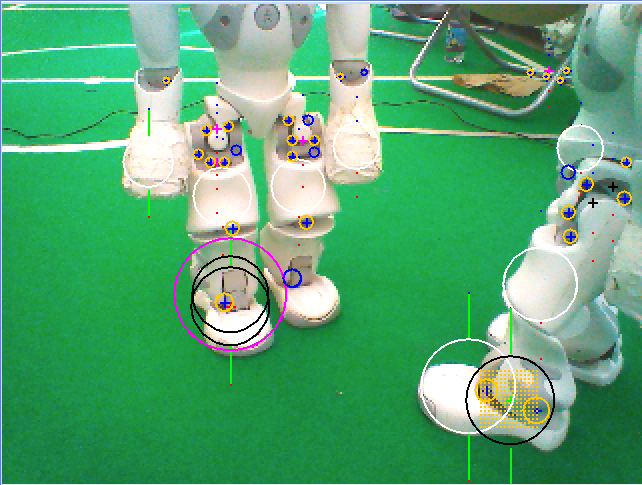
\includegraphics[scale=0.5]{s4.png}
\caption{A record-breaking 25 black spots found in the joints of fellow robots.}
\label{fig:fpBlackSpots}
\end{figure}

\begin{figure}[h]
\centering
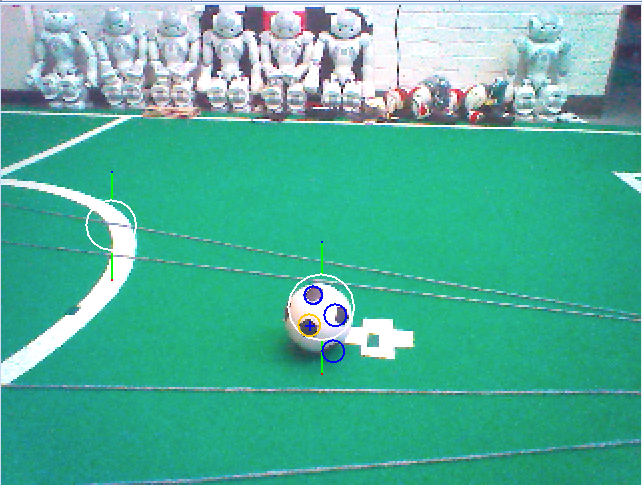
\includegraphics[scale=0.3]{s1.png} \\
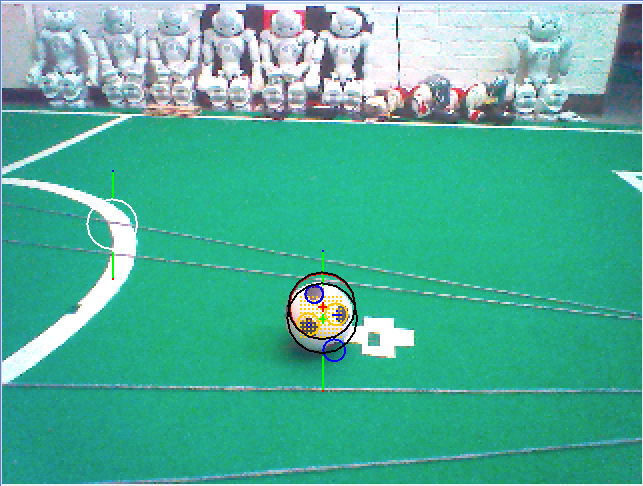
\includegraphics[scale=0.3]{s2.png} \\
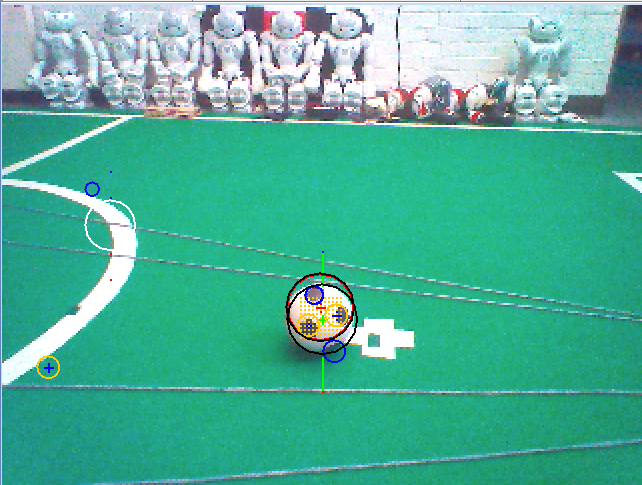
\includegraphics[scale=0.3]{s3.png}
\caption{Three logs taken in the same scenario under lighting conditions of 150 lux. The blue crosses inscribed by yellow circles indicate identified black spots. The red circle (barely visible) in the bottom two images marks a positively identified ball. Note the marked difference in outputs from the ball detector among the three images.}
\label{fig:logs}
\end{figure}

\begin{figure}[h]
\centering
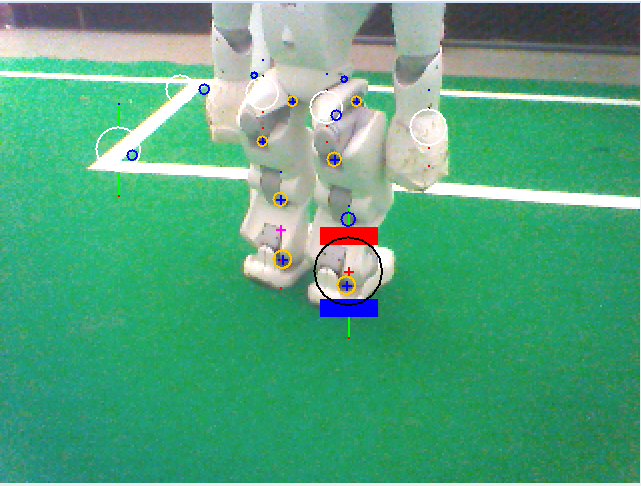
\includegraphics[scale=0.3]{fp1.png} \\
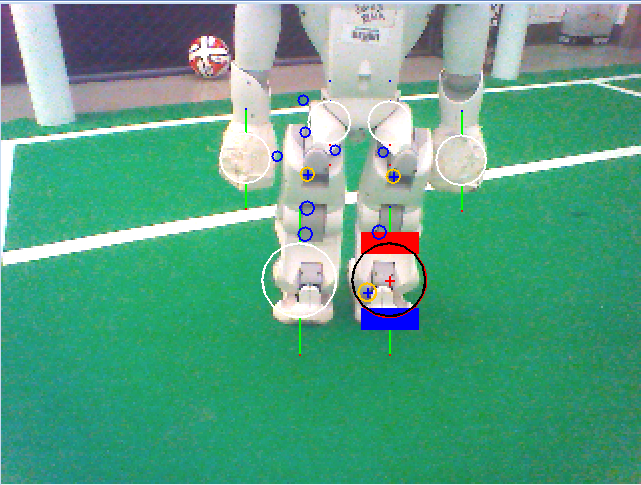
\includegraphics[scale=0.3]{fp2.png} \\
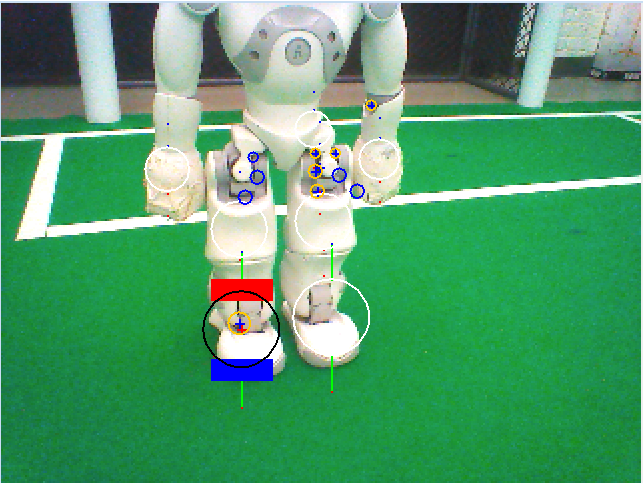
\includegraphics[scale=0.3]{fp3.png}
\caption{False balls detected in the feet and ankles of another robot. The red and blue rectangles indicate the areas checked by the brightness comparison of the regions directly above and below the ball. The hemisphere check was also performed, but is not visualized here. The latter method proved more effective at differentiating true and false positive balls.}
\label{fig:fpballs}
\end{figure}
\pagebreak
\VerbatimInput{code.cpp}
\end{document}